\documentclass{article}

\usepackage{geometry}
\usepackage{xeCJK}
\usepackage{amsmath}
\usepackage{tikz}
\usepackage{pgfplots}
% figure[H] float
\usepackage{float}
\usepackage{amssymb}
\usepackage{hyperref}
\usepackage{setspace}
% 字体底部样式:下划线、波浪线等
\usepackage{ulem}
% 修改公式编号
\usepackage{chngcntr}

% make cdot thicker,比 cdot 更粗的圆点
\makeatletter
\newcommand*\bigcdot{\mathpalette\bigcdot@{.5}}
\newcommand*\bigcdot@[2]{\mathbin{\vcenter{\hbox{\scalebox{#2}{$\m@th#1\bullet$}}}}}
\makeatother

% 设置行间距 1.5 倍
\renewcommand{\baselinestretch}{1.5}
% 自定义图片的标题:Figure -> 图
\renewcommand{\figurename}{图}

% 设置页大小和页边距,或者scale=0.8
\geometry{a4paper,left=3.18cm,right=3.18cm,top=2.54cm,bottom=2.54cm}
% 兼容
\pgfplotsset{compat=1.16}
% 中文默认没有斜体和粗体格式,开启伪斜体和指定黑体;
\setCJKmainfont[AutoFakeSlant, BoldFont=SimHei]{SimSun}
\usetikzlibrary{positioning}
% area of hatch,面积阴影部分
\usetikzlibrary{patterns}
% 箭头类型
\usetikzlibrary{arrows.meta}

\hypersetup{
    colorlinks,
    citecolor=black,
    filecolor=black,
    linkcolor=black,
    urlcolor=black
}
% 定义amsmath arccot
\DeclareMathOperator{\arccot}{arccot}
% 每个章节后,重置公式编号
\counterwithin*{equation}{section}

% 修改公式标签引用颜色
\def\eqref#1{{\color{blue}\hypersetup{linkcolor=blue} (\ref{#1}) }}
% 修改图片标签引用的颜色
\def\figureref#1{{\color{blue}\hypersetup{linkcolor=blue} (\ref{#1}) }}

% 缩进
\usepackage{indentfirst}
\makeatletter
\def\paragraph{
    \parindent2em
}
\makeatother

\begin{document}
  \tableofcontents
  \newpage

  \part{导数与微分}
  \section{导数概念}
    \subsection{导数的引例}
\begin{enumerate}
  \item 速度问题:直线运动的速度
  \item 切线问题:曲线的切线
\end{enumerate}

\subsection{导数的定义}
\subsubsection{函数在一点处的导数与导函数}
\paragraph{}
\textbf{定义~~}设函数 $y = f(x)$ 在点 $x_0$ 的某个邻域内有定义,当自变量 $x$ 在 $x_0$ 处取得增量 $\Delta x$(点 $x_0 + \Delta x$ 仍在该邻域内)时,相应的函数取得增量 $\Delta y = f(x_0 + \Delta x) - f(x_0)$;如果 $\Delta y$ 与 $\Delta x$ 之比当 $\Delta x \to 0$ 时的极限存在,则称函数 $y = f(x)$ 在点 $x_0$ 处\textbf{可导},并称这个极限为函数 $y = f(x)$ 在点 $x_0$ 处的\textbf{导数},记为 $f'(x_0)$,即

\begin{equation}
f'(x_0) = \lim_{\Delta x \to 0} \frac{\Delta y}{\Delta x} = \lim_{\Delta x \to 0} \frac{f(x_0 + \Delta x) - f(x_0)}{\Delta x},
\end{equation}

\paragraph{}
也可记作 $y'|_{x = x_0}, \frac{dy}{dx}|_{x = x_0}$ 或 $\frac{df(x)}{dx}|_{x=x_0}$。

\paragraph{}
也可取不同的形式,常见的有:

\begin{gather}
f'(x_0) = \lim_{h \to 0} \frac{f(x_0 + h) - f(x_0)}{h} , \\
\text{和} \\
f'(x_0) = \lim_{x \to x_0}\frac{f(x) - f(x_0)}{x - x_0}
\end{gather}

\paragraph{}
极限不存在,就说函数 $y = f(x)$ 在点 $x_0$ 处不可导。由于 $\Delta x \to 0$ 时,比式 $\frac{\Delta y}{\Delta x} \to \infty$,函数 $y = f(x)$ 在点 $x_0$ 处导数无穷大。

\paragraph{}
如果函数 $y = f(x)$ 在开区间 $I$ 内的每点处都可导,就称函数 $f(x)$ 在开区间 $I$ 内可导,这就构成了一个新的函数,叫做原来函数 $y = f(x)$ 的导函数,记作 $y', f'(x), \frac{dy}{dx}$ 或 $\frac{df(x)}{dx}$。

\paragraph{}
把 $x_0$ 换成 $x$,即得导函数的定义式:

\begin{gather}
y' = \lim_{x \to 0}\frac{f(x + \Delta x) - f(x)}{\Delta x} , \\
\text{或} \\
f'(x) = \lim_{h \to 0} \frac{f(x + h) - f(x)}{h}.
\end{gather}

\paragraph{}
导函数 $f'(x)$ 简称导数,而 $f'(x_0)$ 是 $f(x)$ 在 $x_0$ 处的导数

\subsubsection{常见函数的导数公式}

\begin{align}
C' &= 0 \qquad \text{(C 为常数)} \\
(x^a)' &= ax^{a-1} \qquad \text{$(a \in Q)$} \\
(\sin x)' &= \cos x \\
(\cos x)' &= - \sin x \\
(e^x)' &= e^x \\
(a^x)' &= a^x \ln a \\
(\ln x)' &= \frac{1}{x} \\
(\log_a x)' &= \frac{1}{x}\log_a e
\end{align}

\subsubsection{单侧导数}
\paragraph{}
极限存在的充分必要条件是左、右极限都\textbf{存在且相等}:

\begin{gather}
\lim_{h \to 0^-}\frac{f(x_0 + h) - f(x_0)}{h} \qquad \text{(左导数)} \\
\lim_{h \to 0^+}\frac{f(x_0 + h) - f(x_0)}{h} \qquad \text{(右导数)}
\end{gather}

\subsection{导数的几何意义}
\paragraph{}
函数 $y = f(x)$ 在点 $x_0$ 处的导数 $f'(x_0)$ 在几何上表示曲线 $y = f'(x)$ 在点 $M(x_0, f(x_0))$ 处的切线的斜率,即:

\begin{equation}
f'(x_0) = \tan \alpha ,
\end{equation}

\paragraph{}
其中 $\alpha$ 是切线的倾角。

\begin{figure}[H]
  \centering
    % 导数的几何意义
\begin{tikzpicture}
  \begin{axis}[xmin=0, xmax=3,ymin=0,ymax=3, grid=none,
    xtick=\empty,ytick=\empty, font=\large, axis lines=middle,
    smooth, xlabel={$x$}, ylabel={$y$}]

    % 曲线
    \addplot[draw=red,domain=0.3:2.5] {(x - 1)^2 + 0.5};
    \node [above] at (axis cs:2,2.5) {$y = f(x_0)$};
    \draw[fill] (1.5,0.75) circle [radius=0.02];
    % 切线
    \addplot[draw=blue,domain=0.3:2.2] {x - 0.75};
    \node [right] at (axis cs:2.2,1.45) {$T$};

    % 辅助线和点
    \addplot[dashed, draw=cyan, mark=none] coordinates {(1.5, 0) (1.5, 0.75)};
    \node [above] at (axis cs:1.5,0.75) {$M$};

    % 倾角
    \draw (1,0) arc (0:45:0.25);
    \node [right] at (axis cs:1,0.1) {$\alpha$};
  \end{axis}
  % 原点
  \node [below left] at (0,0) {$O$};
  \node [below] at (3.45,0) {$x_0$};
\end{tikzpicture}

    \caption{几何意义}
    \label{derivative_geometric_meaning}
\end{figure}

\paragraph{}
过点 $M(x_0, y_0)$ 和切线斜率 $f'(x_0)$,根据直线的点斜式,得到\textbf{切线方程}:

\begin{equation}
y - y_0 = f'(x_0)(x - x_0)
\end{equation}

\paragraph{}
过点 $M(x_0, y_0)$ 和法线斜率 $-\frac{1}{f'(x_0)}, f'(x_0) \neq 0$,根据直线的点斜式,得到\textbf{法线方程}:

\begin{equation}
y - y_0 = - \frac{1}{f'(x_0)}(x - x_0), \; f'(x_0) \neq 0
\end{equation}

\subsection{函数可导性与连续性的关系}
\paragraph{}
设函数 $y = f(x)$ 在点 $x$ 处可导,即

\begin{equation}
\lim_{\Delta x \to 0} \frac{\Delta y}{\Delta x} = f'(x)
\end{equation}

\paragraph{}
存在。由具有极限的函数与无穷小的关系知道,

\begin{equation}
\frac{\Delta y}{\Delta x} = f'(x) + \alpha ,
\end{equation}

\paragraph{}
其中 $\alpha$ 为当 $\Delta x \to 0$ 时的无穷小。上式两边同乘以 $\Delta x$,得

\begin{equation}
\Delta y = f'(x) \Delta x + \alpha\Delta x.
\end{equation}

\paragraph{}
由此可见,当 $\Delta x \to 0$ 时,$\Delta y \to 0$。这就是说,函数 $y = f(x)$ 在点 $x$ 处是连续的。

\paragraph{}
所以,如果函数 $y = f(x)$ 在点 $x$ 处可导,则函数在该点必连续。

\paragraph{}
函数在某点的连续是函数在该点可导的必要条件,但不是充分条件(\textbf{可导即连续,但连续不一定可导})。

\paragraph{}
充分条件:条件 A $\to$ 结论 B,A 则为 B 充分条件

\paragraph{}
必要条件:结论 B $\to$ 条件 A,A 则为 B 必要条件

  \section{函数的求导法则}
    \subsection{函数的和、差、积、商的求导法则}
\paragraph{}
\textbf{定理1~~}如果函数 $u = u(x)$ 及  $v = v(x)$ 都在点 $x$ 具有导数,那么它们的和、差、积、商(除分母为零的点外)都在点 $x$ 具有导数,且

\begin{align}
\left[u(x) \pm  v(x)\right]' &= u'(x) \pm v'(x); \\
\left[u(x)v(x)\right]' &= u'(x)v(x) + u(x)v'(x); \\
\left[\frac{u(x)}{v(x)}\right]' &= \frac{u'(x)v(x) - u(x)v'(x)}{v^2(x)} \; (v(x) \neq 0).
\end{align}

\paragraph{}
定理 1 中的法则(1)、(2)可推广到任意有限个可导函数的情形,即

\begin{align}
(u + v - w)' &= u' + v' - w'; \\
(uvw)' &= u'vw + uv'w + uvw'; \\
(Cu)' &= Cu' \text{~~(C 为常数)}.
\end{align}

\subsection{反函数的求导法则}
\paragraph{}
\textbf{定理2~~}如果函数 $x = f(y)$ 在区间 $I_y$ 内单调、可导且 $f'(y) \neq 0$,则它的反函数 $y = f^{-1}(x)$ 在区间 $I_x = \{x|x = f(x), y \in I_y\}$ 内也可导,且

\begin{equation}
[f^{-1}(x)]' = \frac{1}{f'(y)} \text{~~或~~} \frac{dy}{dx} = \frac{1}{\frac{dx}{dy}}.
\end{equation}

\subsection{复合函数的求导法则}
\paragraph{}
\textbf{定理3~~}如果 $u = g(x)$ 在点 $x$ 可导,而 $y = f(u)$ 在点 $u = g(x)$ 可导,则复合函数 $y = f[g(x)]$ 在点 $x$ 可导,且其导数为

\begin{equation}
\frac{dy}{dx} = f'(u) \cdot g'(x) \text{~~或~~} \frac{dy}{dx} = \frac{dy}{du} \cdot \frac{du}{dx}.
\end{equation}

\subsection{基本求导法则与导数公式}
\subsubsection{常数和基本初等函数的导数公式}

\begin{equation}
  \begin{aligned}[c]
    (C)' &= 0; \\
    (\sin x)' &= \cos x; \\
    (\tan x)' &= \sec^2 x; \\
    (\sec x)' &= \sec x \tan x; \\
    (a^x)' &= a^x\ln a; \\
    (\log_a x)' &= \frac{1}{x \ln a}; \\
    (\arcsin x)' &= \frac{1}{\sqrt{1 - x^2}}; \\
    (\arctan x)' &= \frac{1}{1 + x^2};
  \end{aligned}
  \qquad \qquad
  \begin{aligned}[c]
    (x^\mu)' &= \mu x^{\mu - 1}; \\
    (\cos x)' &= -\sin x; \\
    (\cot x)' &= - \csc^2 x; \\
    (\csc x)' &= -\csc x \cot x; \\
    (e^x)' &= e^x; \\
    (\ln x)' &= \frac{1}{x}; \\
    (\arccos x)' &= - \frac{1}{\sqrt{1 - x^2}}; \\
    (\arccot x)' &= - \frac{1}{1 + x^2}.
  \end{aligned}
\end{equation}

\subsubsection{函数的和、差、积、商的求导法则}
\paragraph{}
设 $u = u(x), v = v(x)$ 都可导,则

\begin{equation}
\begin{aligned}[c]
  (u \pm v)' &= u' \pm v'; \\
  (uv)' & = u'v + uv';
\end{aligned}
\qquad \qquad
\begin{aligned}[c]
  (Cu)' = Cu' \text{~~(C 是常数)}; \\
  \left(\frac{u}{v}\right)' = \frac{u'v - uv'}{v^2}(v \neq 0)
\end{aligned}
\end{equation}

\subsubsection{反函数的求导法则}
\paragraph{}
设 $x = f(y)$ 在区间 $I_y$ 内单调、可导且 $f'(y) \neq 0$,则它的反函数 $y = f^{-1}(x)$ 在区间 $I_x = f(I_y)$ 内也可导,且

\begin{equation}
[f^{-1}(x)]' = \frac{1}{f'(y)} \text{~~或~~} \frac{dy}{dx} = \frac{1}{\frac{dx}{dy}}.
\end{equation}

\subsubsection{复合函数的求导法则}
\paragraph{}
设 $y = f(u)$,而 $u = g(x)$ 且 $f(u)$ 及 $g(x)$ 都可导,则复合函数 $y = f[g(x)]$ 的导数为

\begin{equation}
\frac{dy}{dx} = \frac{dy}{du} \cdot \frac{du}{dx} \text{~~或~~} y'(x) = f'(u) \cdot g'(x).
\end{equation}

  \section{高阶导数}
    \subsection{高阶导数定义}
\paragraph{}
一般的,函数 $y = f(x)$ 的导数 $y' = f'(x)$ 仍然是 $x$ 的函数。我们把 $y' = f'(x)$ 的\textbf{导数}叫做函数 $y = f(x)$ 的\uwave{二阶导数},记作 $y''$ 或 $\frac{d^2y}{dx^2}$,即

\begin{equation}
y'' = (y')' \text{~~或~~} \frac{d^2y}{dx^2} = \frac{d}{dx}(\frac{dy}{dx}).
\end{equation}

\paragraph{}
一般的,$(n - 1)$ 阶导数的导数叫做 \uwave{$n$ 阶导数},记作

\begin{gather}
y^{(n)} \text{~~或~~} \frac{d^ny}{dx^n}.
\end{gather}

\paragraph{}
如果函数 $f(x)$ 在点 $x$ 处具有 $n$ 阶导数,那么 $f(x)$ 在点 $x$ 的某一邻域内必定具有一切低于 $n$ 阶的导数。

\subsection{初等函数的 $n$ 阶导数}

\begin{align}
(e^x)^{(n)} &= e^x \\
(\sin x)^{(n)} &= \sin(x + n \cdot \frac{\pi}{2}) \\
(\cos x)^{(n)} &= \cos(x + n \cdot \frac{\pi}{2}) \\
[\ln(1 + x)]^{(n)} &= (-1)^{n-1}\frac{(n-1)!}{(1+x)^n} \\
(x^{\mu})^{(n)} &= \mu(\mu - 1)(\mu - 2) \cdots (\mu - n + 1)x^{\mu - n} \\
(u \pm v)^{(n)} &= u^{(n)} \pm v^{(n)} \\
(uv)^{(n)} &= u^{(n)}v + nu^{(n - 1)}v' + \frac{n(n-1)}{2!}u^{(n-2)}v'' + \cdots \\
 & \quad + \frac{n(n-1) \cdots (n - k + 1)}{k!} u^{(n - k)}v^{(k)} + \cdots + uv^{(n)} \\
 & = \sum_{k = 0}^{n} C_n^ku^{(n-k)}v^{(k)}. \textbf{~~(Leibniz 公式)}
\end{align}

  \section{隐函数及由参数方程所确定的函数的导数 相关变化率}
    \subsection{隐函数的导数}
\paragraph{}
\textbf{显函数:}等号左端是因变量的符号,而右端是含有自变量的式子,当自变量取定义域内任一值时,由这式子能确定对应的函数值。如:$y = \sin x$。

\paragraph{}
\textbf{隐函数:}如果变量 $x$ 和 $y$ 满足一个方程 $F(x,y) = 0$,在一定条件下,当 $x$ 取某区间内的任一值时,相应的总有满足这方程的\uwave{唯一的} $y$ 值存在,那么方程 $F(x,y) = 0$ 在该区间内确定了一个隐函数。如:$x + y^3 - 1 = 0$。

\paragraph{}
\textbf{隐函数的显化:}把一个隐函数化成显函数。如:$x + y^3 - 1 = 0 \; \to \; y = \sqrt[3]{1 - x}$。

\paragraph{}
\textbf{例子:}求椭圆 $\frac{x^2}{16} + \frac{y^2}{9} = 1$ 在点 $(2, \frac{3}{2}\sqrt{3})$ 处的切线方程。

\paragraph{}
\textbf{解~~}由导数的几何意义知道,所求切线的斜率为
\begin{equation*}
k = y'|_{x = 2}.
\end{equation*}
\paragraph{}
椭圆方程的两边分别对 $x$ 求导(\textbf{y 相当于复合函数,按复合函数求导}),有
\begin{equation*}
\frac{x}{8} + \frac{2}{9}y \cdot \frac{dy}{dx} = 0.
\end{equation*}
\paragraph{}
从而 $\frac{dy}{dx} = -\frac{9x}{16y}.$
\paragraph{}
当 $x = 2$ 时,$y = \frac{3}{2}\sqrt{3}$,代入上式得
\begin{equation*}
\frac{dy}{dx}|_{x = 2} = -\frac{\sqrt{3}}{4}.
\end{equation*}
\paragraph{}
于是所求的切线方程为
\begin{align*}
y - \frac{3}{2}\sqrt{3} &= -\frac{\sqrt{3}}{4}(x - 2), \text{~~即}\\
\sqrt{3}x + 4y - 8\sqrt{3} &= 0.
\end{align*}

\paragraph{}
\textbf{对数求导法~~}在某些场合,先在 $y = f(x)$ 的两边取对数,然后再求出 $y$ 的导数,如:$y = x^{\sin x} (x > 0)$ 的导数,可以先对两边取对数,即 $\ln y = \ln x^{\sin x} = \sin x \cdot \ln x$,然后才对两边求导。

\paragraph{}
对于一般形式的幂指函数

\begin{equation}
y = u^v (u > 0)
\end{equation}

\paragraph{}
如果 $u = u(x), v = v(x)$ 都可导,则,可以表示为:$y = e^{v \ln u}.$

\subsection{由参数方程所确定的函数的导数}
\paragraph{}
研究物体抛射运动轨迹,水平和垂直方向的分解:
\begin{equation}
\left\{
  \begin{array}{l}
    x = v_1 t, \\
    y = v_2 t - \frac{1}{2}gt^2
  \end{array}
\right.
\end{equation}

\paragraph{}
消去参数 $t$,有:

\begin{equation}
y = \frac{v_2}{v_1}x - \frac{g}{2v_1^2}x^2.
\end{equation}

一般的,若\uwave{参数方程}

\begin{equation}
\left\{
\begin{array}{l}
  x = \varphi(t), \\
  y = \psi(t)
\end{array}
\right.
\end{equation}

\paragraph{}
确定 $y$ 与 $x$ 间的函数关系,则称此函数关系所表达的函数为由上面的参数方程确定的函数。

\paragraph{}
如果函数 $x = \varphi(t)$ 具有单调连续反函数 $t = \varphi^{-1}(x)$,且此反函数能与函数 $y = \psi(t)$ 构成复合函数,那么由参数方程所确定的函数可以看成是由函数 $y = \psi(t), t = \varphi^{-1}(x)$ 复合而成的函数 $y = \psi[\varphi^{-1}(x)]$。假设函数 $x = \varphi(t), y = \psi(t)$ 都可导,根据复合函数和反函数的求导法则,有

\begin{align}
\frac{dy}{dx} = \frac{dy}{dt} \cdot \frac{dt}{dx} &= \frac{dy}{dt} \cdot \frac{1}{\frac{dx}{dt}} = \frac{\psi'(t)}{\varphi'(t)} \text{~~即} \\
\frac{dy}{dx} &= \frac{\psi'(t)}{\varphi'(t)}. \\
\text{也可写成~~} \frac{dy}{dx} &= \frac{\frac{dy}{dt}}{\frac{dx}{dt}}.
\end{align}

\paragraph{}
如果 $x = \varphi(t), y = \psi(t)$ 二阶可导,则二阶导数公式为

\begin{equation}
\frac{d^2y}{dx^2} = \frac{\psi''(t)\varphi'(t) - \psi'(t)\varphi''(t)}{\varphi'^3(t)}
\end{equation}

\subsection{相关变化率}
\paragraph{}
设 $x = x(t)$ 及 $y = y(t)$ 都是可导函数,而变量 $x$ 与 $y$ 间存在某种关系,从而变化率 $\frac{dx}{dt}$ 与 $\frac{dy}{dt}$ 间也存在一定关系。这两个相互依赖的变化率称为\uwave{相关变化率}。

\paragraph{}
相关变化率问题研究这两个变化率之间的关系,以便从其中一个变化率求出另外一个变化率。

  \section{函数的微分}
    \subsection{微分的定义}
\paragraph{}
先分析一个具体问题。一块正方形金属薄片受温度变化的影响,其边长由 $x_0$ 变到 $x_0 + \Delta x$,问此薄片的面积改变了多少?

\paragraph{}
设此薄片的边长为 $x$,面积为 $A$,则 $A$ 与 $x$ 存在函数关系:$A = x^2$。薄片受温度变化的影响时面积的改变量,可以看成是当自变量 $x$ 自 $x_0$ 取得增量 $\Delta x$ 时,函数 $A = x^2$ 相应的增量 $\Delta A$,即

\begin{equation}
\Delta A = (x_0 + \Delta x)^2 - x_0^2 = 2x_0\Delta x + (\Delta x)^2.
\end{equation}

\begin{figure}[H]
  \centering
    % 微分例子
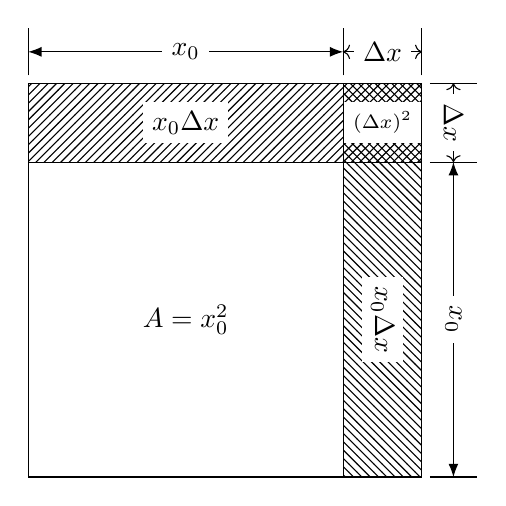
\begin{tikzpicture}
  \draw (0,0) rectangle (5, 5);
  \draw[pattern=north east lines] (0,4) rectangle (5, 5);
  \draw[pattern=north west lines] (4,0) rectangle (5, 5);

  \node at (2,2) {$A = x_0^2$};
  \node[fill=white] at (2,4.5) {$x_0 \Delta x$};
  \node[fill=white, rotate=-90] at (4.5,2) {$x_0 \Delta x$};
  \node[fill=white] at (4.5,4.5) {\scriptsize $(\Delta x)^2$};

  \draw (0, 5.1) -- (0, 5.7);
  \draw (4, 5.1) -- (4, 5.7);
  \draw (5, 5.1) -- (5, 5.7);
  \draw [Latex-Latex] (0, 5.4) -- (4,5.4);
  \node[fill=white] at (2,5.4) {$x_0$};
  \draw [<->] (4, 5.4) -- (5, 5.4);
  \node[fill=white] at (4.5,5.4) {$\Delta x$};

  \draw (5.1, 5) -- (5.7, 5);
  \draw (5.1, 4) -- (5.7, 4);
  \draw (5.1, 0) -- (5.7, 0);
  \draw [<->] (5.4, 5) -- (5.4, 4);
  \node[fill=white,rotate=-90] at (5.4,4.5) {$\Delta x$};
  \draw [Latex-Latex] (5.4, 4) -- (5.4, 0);
  \node[fill=white,rotate=-90] at (5.4,2) {$x_0$};
\end{tikzpicture}

    \caption{金属薄片面积受温度变化}
    \label{金属薄片面积受温度变化}
\end{figure}

\paragraph{}
$\Delta A$ 的第一部分 $2x_0\Delta x$ 是 $\Delta x$ 的线性函数,图中斜线的两个矩形面积之和;第二部分 $(\Delta x)^2$ 在图中带有交叉斜线的小正方形的面积。当 $\Delta x \to 0$ 时,第二部分 $(\Delta x)^2$ 比 $\Delta x$ 高阶无穷小,即 $(\Delta x)^2 = o(\Delta x)$。因此,如果边长改变的很微小,即 $|\Delta x|$ 很小时,面积的改变量 $\Delta A$ 可近似地用第一部分来代替。

\paragraph{}
\textbf{定义~~}设函数 $y = f(x)$ 在某区间内有定义,$x_0$ 及 $x_0 + \Delta x$ 在这区间内,如果增量

\begin{equation}
\Delta y = f(x_0 + \Delta x) - f(x_0)
\end{equation}

\paragraph{}
可表示为

\begin{equation}
\Delta y = A\Delta x + o(\Delta x),
\end{equation}

\paragraph{}
其中 $A$ 是不依赖于 $\Delta x$ 的常数,那么称函数 $y = f(x)$ 在点 $x_0$ 是\uwave{可微}的,而 $A\Delta x$ 叫做函数 $y = f(x)$ 在点 $x_0$ 相应于自变量增量 $\Delta x$ 的\uwave{微分},记作 $dy$,即

\begin{equation}
dy = A\Delta x.
\end{equation}

\paragraph{}
函数 $f(x)$ 在点 $x_0$ 可微的充分必要条件是函数 $f(x)$ 在点 $x_0$ 可导,且当 $f(x)$ 在点 $x_0$ 可微时,其微分一定是

\begin{equation}
dy = f'(x_0)\Delta x.
\end{equation}

\paragraph{}
当 $f'(x_0) \neq 0$ 时,有

\begin{equation}
\lim_{\Delta x \to 0} \frac{\Delta y}{dy} = \lim_{\Delta x \to 0} \frac{\Delta y}{f'(x_0) \Delta x} = \frac{1}{f'(x_0)}\lim_{\Delta x \to 0}\frac{\Delta y}{\Delta x} = 1.
\end{equation}

\paragraph{}
从而,当 $\Delta x \to 0$ 时,$\Delta y$ 与 $dy$ 是等价无穷小,这时有

\begin{equation}
\Delta y = dy + o(dy).
\end{equation}

即$dy$是$\Delta y$ 的\uwave{主部}。又由于$dy = f'(x_0) \Delta x$是$\Delta x$的线性函数,所以在$f'(x_0) \neq 0$的条件下,我们说$dy$是$\Delta y$的\uwave{线性主部}(当$\Delta x \to 0$)。

\paragraph{}
于是,在$f'(x_0) \neq 0$的条件下,以微分$dy = f'(x_0)\Delta x$近似代替增量$\Delta y = f(x_0+\Delta x) - f(x_0)$时,其误差为$o(dy)$。因此,在$|\Delta x|$很小时,有近似等式
\begin{equation}
  \Delta y \approx dy.
\end{equation}

\paragraph{}
函数$y=f(x)$在任意点$x$的微分,称为\uwave{函数的微分},记作$dy$或$df(x)$,即

\begin{equation}
  dy = f'(x)\Delta x.
\end{equation}

\paragraph{}
通常把自变量$x$的增量$\Delta x$称为\uwave{自变量的微分},记作$dx$,即$dx = \Delta x$。于是,函数$y=f(x)$的微分又可记作

\begin{equation}
  dy = f'(x)dx.
\end{equation}

从而有

\begin{equation}
  \frac{dy}{dx} = f'(x).
\end{equation}

\paragraph{}
也就是说,函数的微分$dy$与自变量的微分$dx$之商等于该函数的导数。因此,导数也叫做“\uwave{微商}”。

\subsection{微分的几何意义}
\paragraph{}
在直角坐标系中,函数$y = f(x)$的图形是一条曲线。对于某一固定的$x_0$值,曲线上有一个确定点$M(x_0,y_0)$,当自变量$x$有微小增量$\Delta x$时,就得到曲线上另一点$N(x_0 + \Delta x, y_0 + \Delta y)$。从图\figureref{differential_geometric_meaning}可知:

\begin{align*}
  MQ =&\; \Delta x, \\
  QN =&\; \Delta y.
\end{align*}

过点$M$作曲线的切线$MT$,它的倾角为$\alpha$,则
\begin{equation*}
  QP = MQ \bigcdot \tan{\alpha} = \Delta x \bigcdot f'(x_0),
\end{equation*}
即
\begin{equation*}
  dy = QP.
\end{equation*}

\begin{figure}[H]
  \centering
    % 微分的几何意义
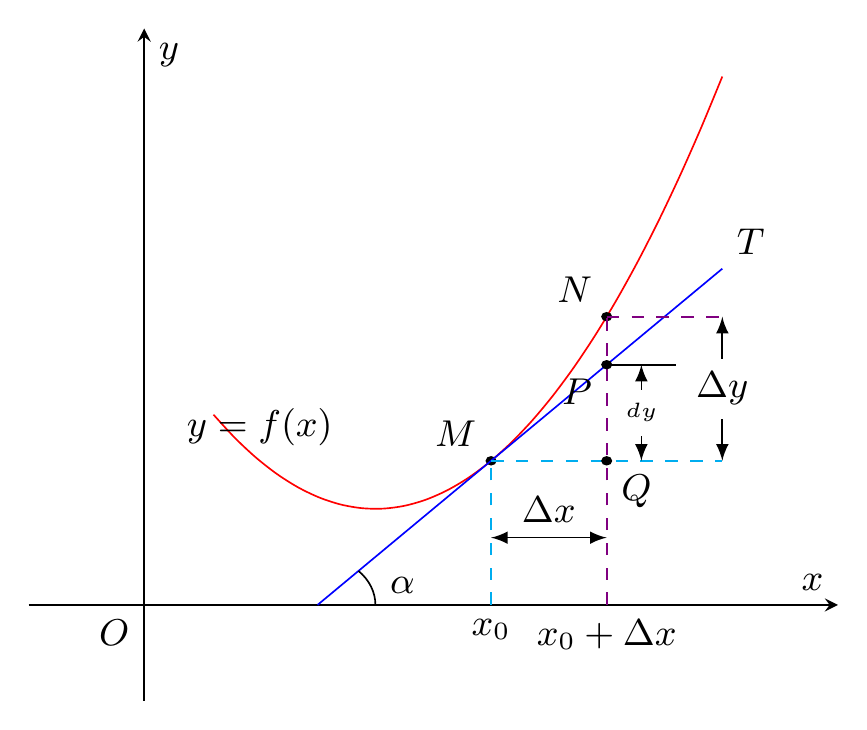
\begin{tikzpicture}[scale = 1.5]
  \begin{axis}[clip=false,xmin=-0.5, xmax=3,ymin=-0.5,ymax=3, grid=none,
    xtick=\empty, ytick=\empty, font=\small, axis lines=middle,
    smooth, xlabel={$x$}, ylabel={$y$}]

    % 曲线
    \addplot[draw=red,domain=0.3:2.5] {(x - 1)^2 + 0.5};
    \node [above] at (0.5,0.75) {$y = f(x)$};
    \draw[fill] (1.5,0.75) circle [radius=0.02];
    \draw[fill] (2,1.5) circle [radius=0.02];
    % 切线
    \addplot[draw=blue,domain=0.75:2.5] {x - 0.75};
    \node [above right] at (2.5,1.75) {$T$};

    % 辅助线和点
    \draw [dashed, draw=cyan] (1.5, 0) -- (1.5, 0.75);
    \draw [dashed, draw=cyan] (1.5, 0.75) -- (2.5, 0.75);
    \node [above left] at (1.5,0.75) {$M$};
    \node [below] at (1.5,0) {$x_0$};

    % \Delta x
    \draw [latex-latex] (1.5, 0.35) -- (2, 0.35);
    \node [above] at (1.75,0.35) {$\Delta x$};

    % \Delta y
    \draw [latex-latex] (2.5, 0.75) -- (2.5, 1.5);
    \node [fill=white] at (2.5,1.125) {$\Delta y$};

    % dy
    \draw (2, 1.25) -- (2.3, 1.25);
    \draw [latex-latex] (2.15, 0.75) -- (2.15, 1.25);
    \node [fill=white, font=\tiny] at (2.15,1) {$dy$};

    \draw [dashed, draw=violet] (2, 0) -- (2, 1.5);
    \draw [dashed, draw=violet] (2, 1.5) -- (2.5, 1.5);
    \node [above left] at (2,1.5) {$N$};
    \node [below] at (2,0) {$x_0 + \Delta x$};

    \draw[fill] (2,1.25) circle [radius=0.02];
    \node [below left] at (2,1.25) {$P$};

    \draw[fill] (2,0.75) circle [radius=0.02];
    \node [below right] at (2,0.75) {$Q$};

    % 倾角
    \draw (1,0) arc (0:45:0.25);
    \node [right] at (1,0.1) {$\alpha$};

    % 原点
    \node [below left] at (0,0) {$O$};
  \end{axis}
\end{tikzpicture}

    \caption{几何意义}
    \label{differential_geometric_meaning}
\end{figure}

\paragraph{}
由此可见,对于可微函数$y=f(x)$而言,当$\Delta y$是曲线$y=f(x)$上的点的纵坐标的增量时,$dy$就是曲线的切线上点的纵坐标的相应增量。

\paragraph{}
当$|\Delta x|$很小时,$|\Delta y - dy|$比$|\Delta x|$小得多。因此在点$M$的邻近,我们可以用切线段来近似代替曲线段。

\paragraph{}
在局部范围内用线性函数近似代替非线性函数,在几何上就是局部用切线段近似代替曲线段,这在数学上称为\textbf{非线性函数的局部线性化},这是微分学的基本思想方法之一。

\subsection{基本初等函数的微分公司与微分运算法则}
\paragraph{}
从函数的微分的表达式
\begin{equation}
  dy = f'(x)dx
\end{equation}
可以看出,要计算函数的微分,只要计算函数的导数,再乘以自变量的微分。因此可得如下的微分公司和微分运算法则。

\subsubsection{基本初等函数的微分公式}
\paragraph{}

\bgroup
\def\arraystretch{1.8}
\setlength\tabcolsep{1.8cm}
\begin{figure}[H]
\centering
  \begin{tabular}{c|c}
    \hline
    导数公式 & 微分公式 \\
    \hline
    $(x^\mu)' = \mu x^{\mu - 1}$ & $d(x^\mu) = \mu x^{\mu - 1}dx$ \\
    $(\sin{x})' = \cos{x}$ & $d(\sin{x}) = \cos{x}dx$ \\
    $(\cos{x})' = -\sin{x}$ & $d(\cos{x}) = -\sin{x}dx$ \\
    $(\tan{x})' = \sec^2{x}$ & $d(\tan{x}) = \sec^2{x}dx$ \\
    $(\cot{x})' = -\csc^2{x}$ & $d(\cot{x}) = -\csc^2{x}dx$ \\
    $(\sec{x})' = \sec{x}\tan{x}$ & $d(\sec{x}) = \sec{x}\tan{x}dx$ \\
    $(\csc{x})' = -\csc{x}\cot{x}$ & $d(\csc{x}) = -\csc{x}\cot{x}dx$ \\
    $(a^x)' = a^x\ln{a}$ & $d(a^x) = a^x\ln{a}dx$ \\
    $(e^x)' = e^x$ & $d(e^x) = e^xdx$ \\
    $(\log_a{x})' = \frac{1}{x\ln{a}}$ & $d(\log_a{x}) = \frac{1}{x\ln{a}}dx$ \\
    $(\ln{x})' = \frac{1}{x}$ & $d(\ln{x}) = \frac{1}{x}dx$ \\
    $(\arcsin{x})' = \frac{1}{\sqrt{1-x^2}}$ & $d(\arcsin{x}) = \frac{1}{\sqrt{1-x^2}}dx$ \\
    $(\arccos{x})' = -\frac{1}{\sqrt{1-x^2}}$ & $d(\arccos{x}) = -\frac{1}{\sqrt{1-x^2}}dx$ \\
    $(\arctan{x})' = \frac{1}{\sqrt{1+x^2}}$ & $d(\arctan{x}) = \frac{1}{\sqrt{1+x^2}}dx$ \\
    $(\arccot{x})' = -\frac{1}{\sqrt{1+x^2}}$ & $d(\arccot{x}) = -\frac{1}{\sqrt{1+x^2}}dx$ \\
    \hline
  \end{tabular}
\end{figure}
\egroup

\subsubsection{函数和、差、积、商的微分法则}
\paragraph{}
由函数和、差、积、商的求导法则,可推得相应的微分法则,表中$u = u(x), v = v(x)$都可导。

\bgroup
\def\arraystretch{2}
\setlength\tabcolsep{1.2cm}
\begin{figure}[H]
\centering
  \begin{tabular}{c|c}
    \hline
    函数和、差、积、商的求导法则 & 函数和、差、积、商的微分法则 \\
    \hline
    $(u \pm v)' = u' \pm v'$ & $d(u \pm v) = du \pm dv$ \\
    $(Cu)' = Cu'$ & $d(Cu) = Cdu$ \\
    $(uv)' = u'v + uv'$ & $d(uv) = vdu + udv$ \\
    $(\frac{u}{v})' = \frac{u'v - uv'}{v^2} \;(v \neq 0)$ & $d(\frac{u}{v}) = \frac{vdu - udv}{v^2} \;(v \neq 0)$ \\
    \hline
  \end{tabular}
\end{figure}
\egroup

\subsubsection{复合函数的微分法则}
\paragraph{}
设$y = f(u)$及$u = g(x)$都可导,则复合函数$y=f[g(x)]$的微分为
\begin{equation}
  dy = y'_x dx = f'(u)g'(x)dx.
\end{equation}
由于$g'(x)dx = du$,所以,复合函数$y = f[g(x)]$的微分公式也可以写成
\begin{equation}
  dy = f'(u)du \; \text{或} \; dy = y'_u du.
\end{equation}

\paragraph{}
由此可见,无论$u$是自变量还是中间变量,微分形式$dy = f'(u)du$保持不变,这一性质称为\textbf{微分形式不变性}。这性质表示,当变换自变量时,微分形式$dy = f'(u)du$并不改变。

\subsection{微分在近似计算中的应用}
\subsubsection{函数的近似计算}
\paragraph{}
在工程问题中,经常会遇到一些复杂的计算公式。如果直接用这些公式进行计算,那是很费力的。利用微分往往可以把一些复杂的计算公式用简单的近似公式来代替。
\paragraph{}
前面说过,如果$y = f(x)$在点$x_0$处的导数$f'(x_0) \neq 0$,且$|\Delta x|$很小时,我们有
\begin{equation}
  \label{函数的近似计算例子1}
  \Delta y \approx dy = f'(x_0)\Delta x.
\end{equation}
这个式子也可以写成
\begin{equation}
  \label{函数的近似计算例子2}
  \Delta y = f(x_0 + \Delta x) - f(x_0) \approx f'(x_0)\Delta x,
\end{equation}
或
\begin{equation}
  \label{函数的近似计算例子3}
  f(x_0 + \Delta x) \approx f(x_0) + f'(x_0)\Delta x.
\end{equation}
在\eqref{函数的近似计算例子3}式中令$x = x_0 + \Delta x$,即$\Delta x = x - x_0$,那么\eqref{函数的近似计算例子3}式可改写为
\begin{equation}
  \label{函数的近似计算例子4}
  f(x) \approx f(x_0) + f'(x_0)(x-x_0).
\end{equation}

\paragraph{}
如果$f(x_0)$与$f'(x_0)$都容易计算,那么可利用\eqref{函数的近似计算例子2}式来近似计算$\Delta y$,利用\eqref{函数的近似计算例子3}式来近似计算$f(x_0 + \Delta x)$,或利用\eqref{函数的近似计算例子4}式来近似计算$f(x)$。

\paragraph{}
这种近似计算的实质就是用$x$的线性函数$f(x_0) + f'(x_0)(x-x_0)$来近似表达函数$f(x)$。从导数的几何意义[图\figureref{differential_geometric_meaning}]可知道,这也就是用曲线$y=f(x)$在点$(x_0, f(x_0))$处的切线来近似代替该曲线(就切点邻近部分来说)。

\subsubsection{误差估计}
\paragraph{}
例如,计算圆钢的截面积$A$,可先用卡尺测量圆钢截面的直径$D$,然后根据公式$A = \frac{\pi}{4}D^2$算出$A$。

\paragraph{}
由于测量仪器的精度、测量的条件和测量的方法等各种因素的影响,测得的数据往往带有误差,而根据带有误差的数据计算,所得的结果也会有误差,我们把它叫做\uwave{间接测量误差}。

\paragraph{}
可以通过微分来估计间接测量误差。

\paragraph{}
如果某个量的精确值为$A$,它的近似值为$a$,那么$|A-a|$叫做$a$的\uwave{绝对误差}。而绝对误差与$|a|$的比值$\frac{|A-a|}{|a|}$叫做$a$的\uwave{相对误差}。

\paragraph{}
在实际工作中,某个量的精确值往往是无法知道的,于是绝对误差和相对误差也就无法求得。但是根据测量仪器的精度等因素,有时能够确定误差在某一个范围内。

\paragraph{}
如果某个量的精确值是$A$,测得它的近似值是$a$,又知道它的误差不超过$\delta_A$,即
\begin{equation}
  |A-a| \leq  \delta_A,
\end{equation}
那么$\delta_A$叫做测量$A$的\uwave{绝对误差限},而$\frac{\delta_A}{|a|}$叫做测量$A$的\uwave{相对误差限}。

\paragraph{}
一般的,根据直接测量的$x$值按公式$y=f(x)$计算$y$值时,如果已知测量$x$的绝对误差限是$\delta_x$,即
\begin{equation}
  |\Delta x| \leq \delta_x,
\end{equation}
那么,当$y' \neq 0$时,$y$的绝对误差
\begin{equation}
  |\Delta y| \approx |dy| = |y'| \bigcdot |\Delta x| \leq |y'| \bigcdot \delta_x,
\end{equation}
即$y$的绝对误差限约为
\begin{equation}
  \delta_y = |y'| \bigcdot \delta_x;
\end{equation}
$y$的相对误差限约为
\begin{equation}
  \frac{\delta_y}{|y|} = |\frac{y'}{y}| \bigcdot \delta_x.
\end{equation}

\paragraph{}
以后常把绝对误差限与相对误差限简称为\uwave{绝对误差}与\uwave{相对误差}。

\end{document}
